\documentclass[12pt]{article}
\usepackage[T1]{fontenc}
\usepackage[utf8]{inputenc}
\usepackage[a4paper, margin=2cm]{geometry} % Adjusted geometry
\usepackage{graphicx}
\usepackage{multicol} % Include multicol package for multiple columns
\usepackage[backend=biber, style=apa, citestyle=apa]{biblatex} % Combined biblatex setup
\addbibresource{references.bib} % Ensure this matches your actual .bib file name

\usepackage{hyperref}
\usepackage{amsmath}
\usepackage{amsfonts}
\usepackage{amssymb}
\usepackage{booktabs} % For formal tables


\title{Swing Probability Prediction in Baseball using Pitch Characteristics and Game Context}

\author{Olubayode Ebenezer \\ \\ Msc. Sports Data Analytics\\ 
\\Data Science in Economics}

\date{Spring Semester \today}




\begin{document}

\maketitle


\begin{abstract}
This research focuses on predictive modeling of baseball swing probabilities using advanced machine learning techniques, specifically targeting the first phase of a broader study that includes econometric analyses. This phase utilizes a hybrid ensemble approach, combining LGBM and XGBCatboost classifiers to address sports analytics challenges such as class imbalance and prediction accuracy. The machine learning aspect of the study has significantly enhanced prediction accuracy, as evidenced by improvements in the F1 score and overall model accuracy, demonstrating the model's robust generalization capabilities across various game scenarios. While the econometric analysis is still underway, this work highlights the efficacy of integrating multiple sophisticated machine learning models to achieve precise and reliable predictions, crucial for strategic decision-making in sports. This abstract underscores the practical applications of such analytical methods in refining coaching techniques and strategic game management within the realm of baseball and other sports analytics.
\end{abstract}

\section{Introduction}
This work applies a combination of machine learning and econometric techniques to study baseball swing probabilities, aiming to enhance the understanding of player decisions during games and explore broader economic implications. By building on the advanced analytical approaches exemplified by \cite{Deshpande2023}, this project seeks to extend the frontier of baseball analytics. The integration of these techniques is intended to deepen the strategic aspects of the game and improve coaching and player performance through data-driven insights.

\subsection{Machine Learning and Econometrics in Baseball Analytics}
The study by \cite{Deshpande2023} highlights the potential of sophisticated statistical models, like Bayesian Additive Regression Trees (BART), to capture the complex dynamics of baseball, including the interplay of various game-state variables. Leveraging similar complexity, this project initially employs machine learning to develop robust predictive models of swing probability. These models will consider not just pitch location and type but will also integrate broader game context, player performance metrics, and situational pressures—factors that significantly influence a player's decision to swing. The decision to use machine learning in the initial phase of this project is justified by the need for a highly adaptive and predictive framework capable of handling the vast and varied data sources typical in baseball, including high-dimensional player and game-state characteristics. Machine learning models excel in identifying patterns and making predictions from complex datasets, thus providing a solid foundation for the subsequent econometric analysis.

\subsection{Econometric Analysis Phase}
The second phase of this project will explore the economic implications of swing decisions using econometric models to assess the effects of pitch types, speeds, or game situations on swing probabilities. This approach aims to provide insights valuable for training strategy and player development in baseball, thereby enhancing the quality of this work. Such analysis could impact a player's career longevity, contract value, and the team's financial performance, contributing not only to the tactical aspects of baseball but also to strategic management and economic evaluation within the sport. However, this paper will only focus on the first phase which is the building of predictive machine learning model for swing probability.


\maketitle

\section{Literature Review}

\subsection*{Review of Related Studies}
Recent studies, such as those by \cite{DeRenne2007} and \cite{Escamilla2009a}, have focused on the spatial characteristics of successful baseball swings and their correlation with skill level, but few have delved deeply into the temporal characteristics, which are crucial for optimizing batting performance. Notably, skilled hitters exhibited earlier initiation of the shifting, stepping, and landing phases, which allowed for a more controlled and powerful swing (\cite{Nakata2013}; \cite{Escamilla2009a}). This understanding is invaluable for coaches, who can use this knowledge to train athletes more effectively, ensuring that they initiate each swing phase in an optimal sequence to maximize performance.

\subsection{Biomechanical Insights and Swing Prediction}
Fortenbaugh (2011) work on the biomechanics of the baseball swing provides critical insights into the factors influencing batting performance by analyzing biomechanical data from AA-level Minor League Baseball players. The study details how kinematic and kinetic variables change with different pitch types and locations. This biomechanical understanding is foundational for developing more accurate swing probability models. Fortenbaugh identifies several key phases of the swing: stance, stride, coiling, swing initiation, swing acceleration, and follow-through, which are delineated by distinct biomechanical events. Each phase involves specific movements and forces that can be quantitatively described and used to predict the swing probability.

\subsection*{Enhancing Coaching Strategies and Player Performance}
The actionable insights derived from the predictive model are intended to transform coaching strategies and player performance. By quantifying the impact of various factors on swing probabilities, coaches can tailor their training programs more effectively, focusing on improving decision-making skills under different game conditions. Additionally, players can benefit from personalized feedback on their performance, helping them to adjust their strategies in real-time, much like the detailed case study provided by \cite{Deshpande2023} on Mike Trout.

\subsection{Integration of Advanced Analytical Techniques}
Previous works build on Bayesian methods by \cite{Deshpande2023} critiques traditional metrics that oversimplify swing decisions. The works only focus on Strike Zone primarily assessing whether a pitch is inside or outside the strike zone, prompting batters to swing at pitches within and refrain from those outside (\cite{Slowinski2010}). This approach overlooks critical factors such as the type of pitch, its speed, and historical interactions between pitcher and batter, which can significantly influence the batter’s decision to swing. The integration of variables beyond traditional metrics, such as the Strike Zone—assessing whether a pitch is inside or outside the strike zone—such as game situation, psychological variables, and other temporal and kinematic data, will contributes to enhancing hitting performance. This explains why this research would contribute to baseball analytics as it would incorporate game situations variables unlike the traditional approach.

\subsection{Predictive Models and Swing Probability}
Understanding and predicting swing probability is crucial due to the complex, highly coordinated nature of batting. The ability to accurately predict when a batter will swing, considering varying pitch types and locations, significantly enhances player training and game strategy. Batting is recognized as one of the most challenging skills in sports, requiring sophisticated analytical techniques to improve performance and decision-making processes.

\subsection{Influence of Pitch Characteristics on Swing Decisions}
Fortenbaugh (2011) reveals significant biomechanical adaptations in response to different pitch locations and speeds. For instance, swings against inside pitches are characterized by greater pelvis rotation, a factor that could be crucial in predicting swings in real-time. Incorporating pitch characteristics into predictive models can enhance their accuracy, providing coaches and players with actionable insights that can transform training strategies and player performance.

\maketitle

\section{Data Source and Utilization}

\textbf{Source:} \\
Dataset Description: The data consists of comprehensive pitch data from the Miami Marlins over three seasons. This dataset includes every pitch thrown in games during these seasons, providing a rich source of information for analysis. This data has been collected through the data strategy team used during, ensuring accuracy and reliability.

\textbf{Utilization Strategy:} \\
\begin{itemize}
    \item \textbf{Training Data:} The first two seasons of data will be used to train the predictive model. This approach allows the model to learn from a substantial set of examples, covering a wide range of game situations and pitcher-batter matchups.
    \item \textbf{Validation Data:} The third season of data will serve as the validation set. This set will test the model’s predictive power and generalizability to new, unseen data, ensuring that the model remains effective outside of the training sample. It doesn’t have the descriptions columns like the first two seasons data that have it.
\end{itemize}

\textbf{Key Data Columns and Their Importance:}

\begin{itemize}
    \item \textbf{Pitch-Specific Data:}
    \begin{itemize}
        \item \textbf{pitch\_id:} Serves as a unique identifier for each pitch, crucial for data management and tracking individual pitches throughout the analysis.
        \item \textbf{descriptions:} Contains textual descriptions of the outcome of each pitch (e.g., strike, ball, hit, or foul), which are essential for labeling the data in supervised learning scenarios. This description column was used combined with my knowledge of baseball to generate the Y label called SwingType which was not given in all the datasets.
        \item \textbf{release\_speed:} The speed at which the pitch leaves the pitcher’s hand, measured in miles per hour. This is a critical factor in predicting the batter’s reaction time and the likelihood of different types of swings.
        \item \textbf{pitch\_type:} A coded categorization of the pitch. Different pitch types behave differently in terms of trajectory and speed, influencing batter decisions significantly.
    \end{itemize}
    \item \textbf{Batter and Pitcher Specifics:}
    \begin{itemize}
        \item \textbf{batter:} Identifier for the batter facing the pitch, important for analyzing batter-specific performance and tendencies.
        \item \textbf{pitcher:} Identifier for the pitcher throwing the ball, used to analyze pitcher-specific strategies and effectiveness.
        \item \textbf{stand:} Indicates whether the batter stands on the left or right side of the plate, affecting how they perceive and react to pitches.
        \item \textbf{p\_throws:} Specifies whether the pitcher throws with their left or right hand, which impacts pitch dynamics and batter response.
    \end{itemize}
    \item \textbf{Pitch Trajectory and Location:}
    \begin{itemize}
        \item \textbf{pfx\_x and pfx\_z:} Measurements of the pitch’s lateral (x) and vertical (z) movement as it approaches the plate. These metrics are crucial for understanding the behavior of different pitches and their deception levels.
        \item \textbf{plate\_x and plate\_z:} Exact horizontal (x) and vertical (z) positions where the pitch crosses home plate. This data helps determine whether a pitch is likely to be called a strike or a ball.
        \item \textbf{sz\_top and sz\_bot:} Defines the top and bottom boundaries of the strike zone as the pitch crosses the plate. These are key for assessing the accuracy and control of the pitcher and for modeling the strike zone dynamically based on the batter’s stance and size.
    \end{itemize}
    
\end{itemize}

\maketitle

\section{Method}

This section discusses the methodology and approach used in developing a predictive model for Swing Probability. A comprehensive data analysis and preparation phase was undertaken, analyzing over two million pitches from two different seasons of Miami Marlins' games. This phase involved pattern analysis that influences swing decisions, meticulous data cleaning to isolate relevant features, and addressing class imbalance to ensure robust model training.

\subsection{Feature Engineering and Model Development}
The feature engineering phase refined the approach through polynomial interactions and statistical methods to enhance feature relevance and interactions. Strategic use of feature importance metrics helped select the most informative variables. This selective refinement ensured that the model inputs were accurate and pivotal in determining swing probabilities. The model development and tuning stage involved constructing a predictive model using the historically significant data collected. Extensive hyperparameter tuning was crucial for adapting the model to the nuances of baseball pitching and batting interactions, preventing overfitting and optimizing performance.

\subsection{Validation and Evaluation}
Validation and evaluation of the model were rigorously executed through cross-validation strategies, testing the model’s robustness and accuracy across different subsets of the data. The model's effectiveness was primarily assessed using the F1 Score, balancing precision and recall—key for dealing with the previously identified class imbalances. The validated model was then applied to the third season's data, which lacked direct pitch outcome information, to test its practical utility. This application demonstrated the model's ability to predict swing decisions accurately, providing significant insights for baseball teams and analysts.

\subsection{Assumptions Criteria for Creating the Y Label}
The "SwingLikelihood" category was created from the "descriptions" columns, based on a systematic approach informed by a detailed understanding of baseball rules and typical outcomes of pitches. Here's a breakdown of the assumptions and criteria used:

\subsubsection{Logical Grouping Based on Baseball Dynamics}
\begin{itemize}
    \item \textbf{Unlikely Swing:} Includes Balls and Called Strikes where no swing is attempted.
    \item \textbf{No Swing:} Includes Blocked Balls, Hit By Pitches, and Pitchouts where no swing occurs.
    \item \textbf{Definite Swing:} Encompasses Foul, Hit Into Play, Swinging Strike, Foul Tip, and Swinging Strike (Blocked).
    \item \textbf{Attempt to Swing (bunt):} Includes Foul Bunt, Missed Bunt, and Bunt Foul Tip.
\end{itemize}

\subsubsection{Handling Anomalies}
\begin{itemize}
    \item \textbf{Foul\_Pitchout:} A rare description suggesting an attempted pitchout where the batter decided to swing, likely due to a misjudgment, leading to a foul.
\end{itemize}

\subsubsection{Classification into General SwingProbability}
\begin{itemize}
    \item \textbf{Swing:} Includes all outcomes where a swing was clearly intended or occurred.
    \item \textbf{No Swing:} Encompasses outcomes where the batter typically does not swing.
      
\end{itemize}
    
These criteria ensure that the model's input reflects realistic baseball situations and batter decisions, improving the predictive accuracy of swing likelihood and supporting strategic decision-making.

\begin{center}
    
% \end{center}
        \centering
        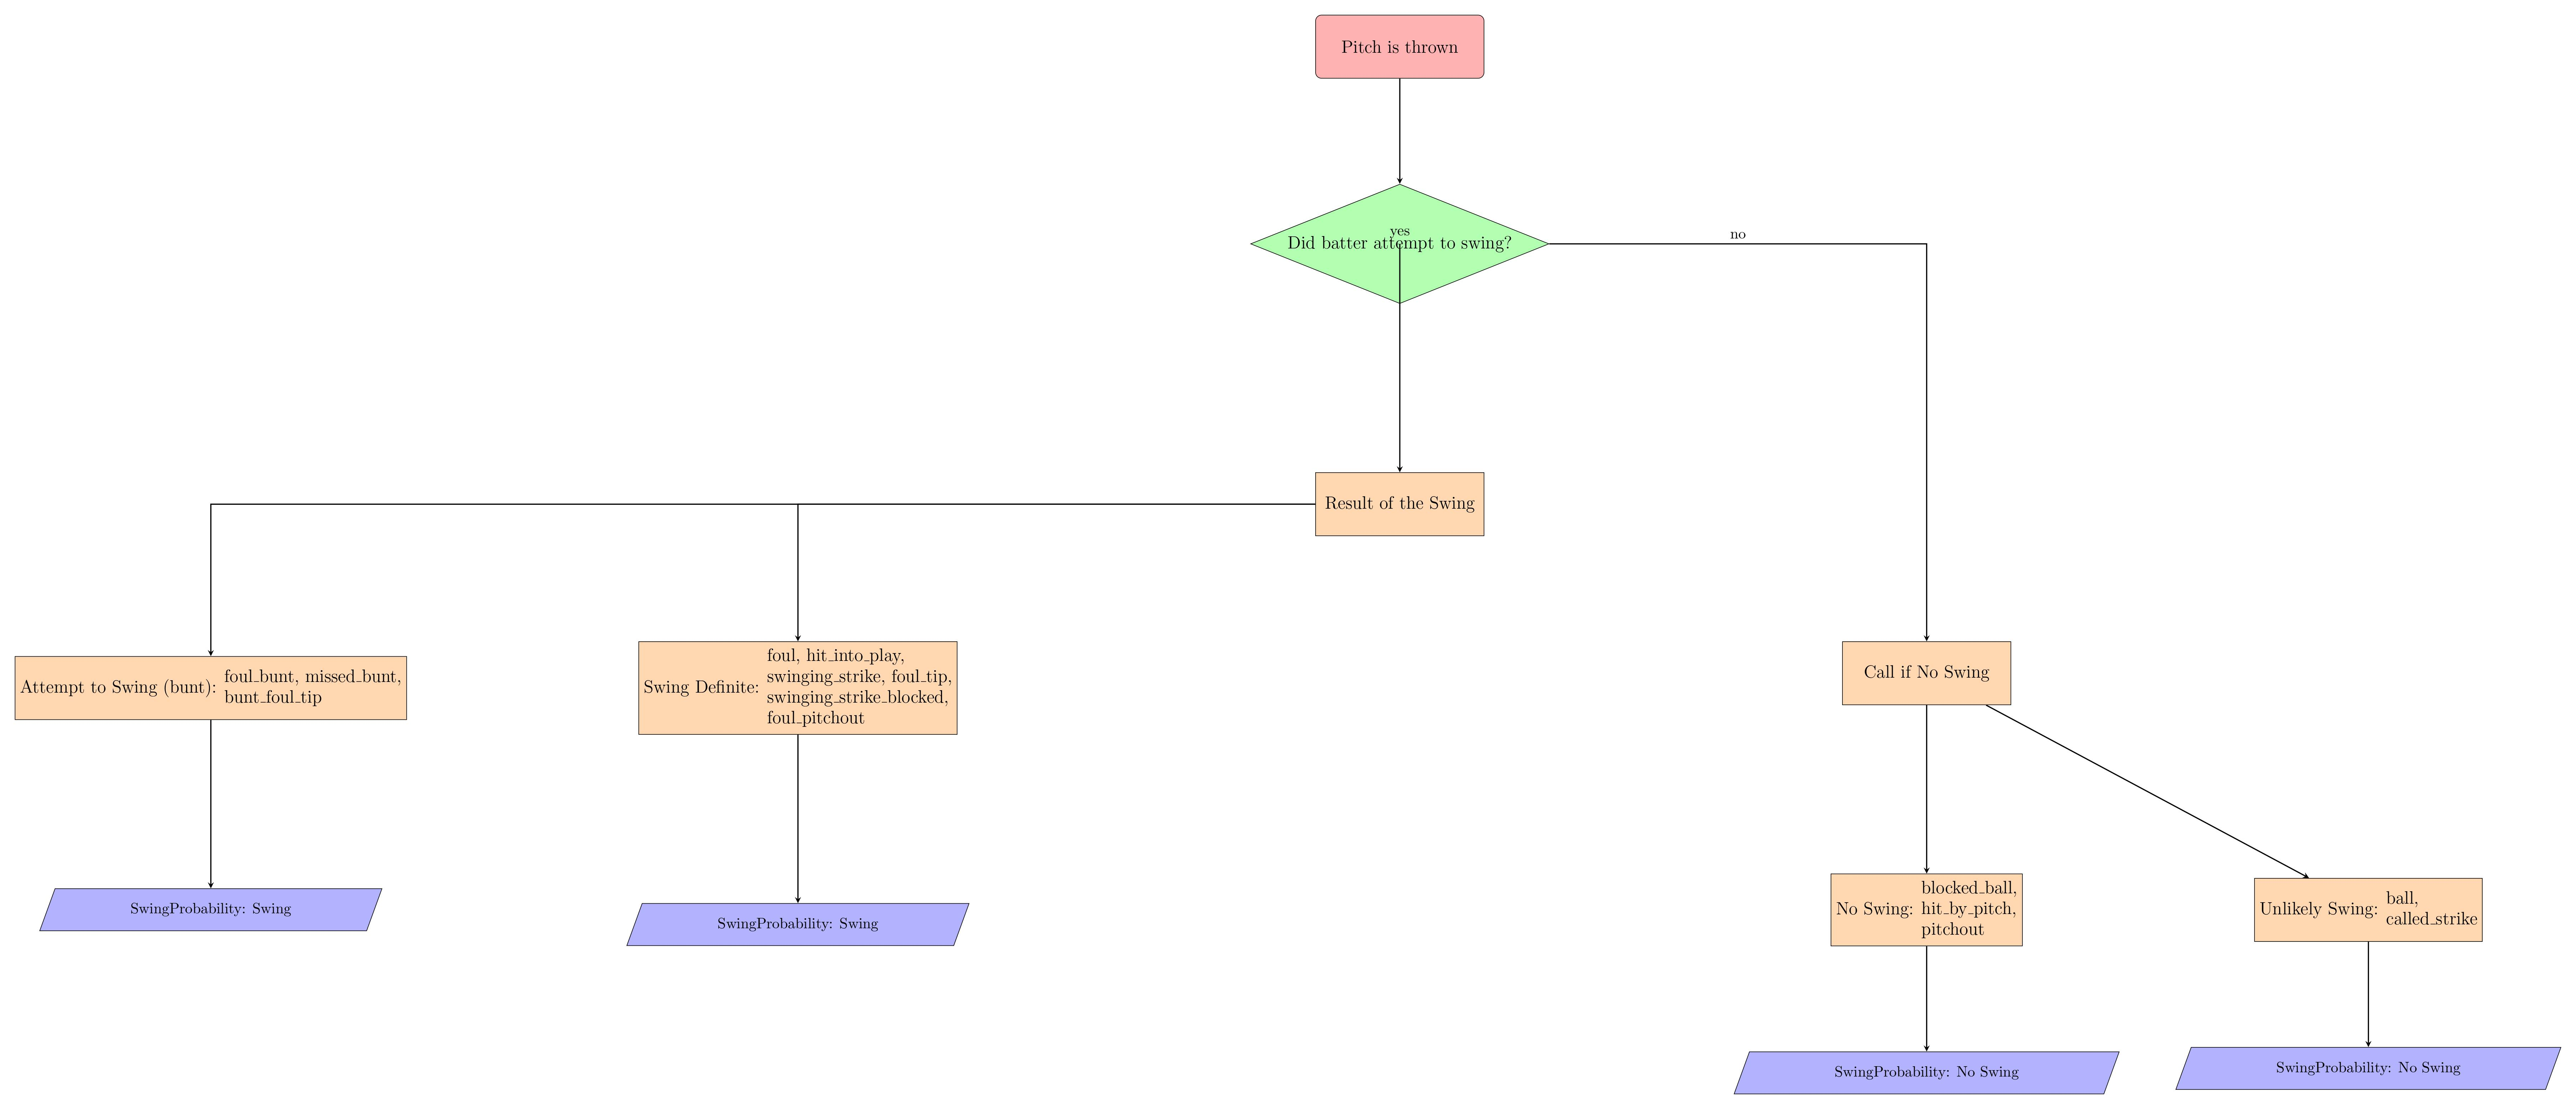
\includegraphics[width=0.8\textwidth]{flow_chart (2).jpg} % Adjust the path to your image
        \textbf{\\Figure 1} Diagram of criteria used in Producing the SwingProbability Y Label Column.
        
\end{center}


\section{Data Pre-Processing}

\subsection{Data Quality Assessment}
In preparing the dataset for predictive modeling on swing probabilities using extensive pitch data, a comprehensive quality assessment was performed to ensure the robustness and accuracy of the analysis. The data quality report revealed a varied landscape of missing values across different variables, each with significant implications for modeling strategies.

\subsubsection{Assessment of Missing Values}
The two seasons of pitch data were combined into a single data frame, enabling a unified analysis platform. The assessment highlighted that certain columns, such as \textit{pfx\_x}, \textit{pfx\_z}, \textit{sz\_bot}, \textit{plate\_z}, \textit{release\_speed}, \textit{sz\_top}, and \textit{plate\_x}, exhibited missing values, with percentages ranging from approximately 0.05\% to 0.24\%. Notably, \textit{pfx\_x} and \textit{pfx\_z}, which measure the lateral and vertical movement of pitches, had the highest missing rates at 0.24\% and 0.10\%, respectively, indicating potential issues in capturing complete data for pitch movement, which is crucial for understanding pitch dynamics.

Columns like \textit{pitch\_id} and \textit{pitch\_type} also showed missing values, though less prevalent, which could affect the identification and categorization of pitches in analyses. The presence of missing values in \textit{release\_speed}, \textit{sz\_top}, and \textit{sz\_bot} suggests gaps in capturing essential pitch characteristics and batter-specific strike zone data.

\subsubsection{Classification of Missing Data}
Some of these missing data are classified as Missing At Random (MAR) because the missingness of the data is related to observed variables but not to the missing values themselves. Conversely, a few, such as \textit{Pitch\_id}, are classified as Missing Not At Random (MNAR) because the missingness of the \textit{pitch\_id} is related to the missing values themselves, even accounting for observed variables.

\subsubsection{Completeness of Other Variables}
Conversely, variables such as \textit{balls}, \textit{strikes}, \textit{p\_throws}, \textit{stand}, \textit{description}, \textit{pitcher}, \textit{batter}, and \textit{season} recorded no missing values, indicating comprehensive data capture for these aspects. This completeness is vital, as these variables play critical roles in determining the context of each pitch and its likely outcome.

The dataset also exhibited a broad range of unique values across columns, reflecting the diversity of events in baseball pitching and batting interactions. For example, the \textit{pitch\_id} column had over 1.4 million unique entries, confirming the extensive granularity of the data. See Table 1:

\section*{Quality Report of the Two Season Dataset}

\begin{table}[h]
\centering
% \sisetup{
%   table-format=7.0, 
%   round-mode=places, 
%   round-precision=6, 
%   group-four-digits=true
% }
\begin{tabular}{
  @{} 
  l 
  S[table-format=6.0] 
  S[table-format=1.6]
  S[table-format=7.0] 
  l 
  @{}
  }
\toprule
\textbf{Column} & {\textbf{Total NaN}} & {\textbf{Percent of NaN}} & {\textbf{Nunique}} & \textbf{Dtype} \\ 
\midrule
pfx\_x          & 3460                & 0.243938                 & 482               & float64        \\
pitch\_id       & 1611                & 0.113579                 & 1416781           & float64        \\
pfx\_z          & 1477                & 0.104132                 & 451               & float64        \\
sz\_bot         & 824                 & 0.058094                 & 143               & float64        \\
plate\_z        & 812                 & 0.057248                 & 999               & float64        \\
release\_speed  & 779                 & 0.054921                 & 681               & float64        \\
sz\_top         & 779                 & 0.054921                 & 181               & float64        \\
plate\_x        & 779                 & 0.054921                 & 827               & float64        \\
pitch\_type     & 740                 & 0.052172                 & 16                & object         \\
balls           & 0                   & 0.000000                 & 5                 & int64          \\
strikes         & 0                   & 0.000000                 & 4                 & int64          \\
p\_throws       & 0                   & 0.000000                 & 2                 & object         \\
stand           & 0                   & 0.000000                 & 2                 & object         \\
description     & 0                   & 0.000000                 & 14                & object         \\
pitcher         & 0                   & 0.000000                 & 1168              & int64          \\
batter          & 0                   & 0.000000                 & 1227              & int64          \\
season          & 0                   & 0.000000                 & 2                 & int64          \\
\bottomrule
\end{tabular}
\caption{Detailed Quality Report of Dataset Variables}
\end{table}


\maketitle

\section{Handling Missing Values}

Given the importance of a complete dataset for accurate predictive modeling, the following strategies were implemented to address missing values:

\subsection*{Release Speed (release\_speed)}
\textbf{Strategy:} Missing values in \textit{release\_speed} were imputed using the median value grouped by \textit{pitch\_type}. This approach leverages the characteristic speed ranges associated with different types of pitches, providing a contextually relevant method for estimating missing speeds.

\subsection*{Plate Coordinates (plate\_x and plate\_z)}
\textbf{Strategy:} Missing values in the horizontal (plate\_x) and vertical (plate\_z) locations where the pitch crosses home plate were filled by computing the mean values grouped by \textit{pitch\_type} and \textit{release\_speed}. This method assumes that pitches of a specific type and speed tend to follow similar trajectories, making the mean a suitable estimator for missing data points.

\subsection*{Strike Zone Dimensions (sz\_top and sz\_bot)}
\textbf{Strategy:} To address missing values in the top (sz\_top) and bottom (sz\_bot) of the strike zone, the median values were imputed based on \textit{pitch\_type}. This strategy is predicated on the assumption that different pitch types generally maintain consistent strike zone dimensions due to their typical delivery mechanics. The median was chosen as the central measure due to the non-normal distribution of these dimensions across different pitches and batters.

This systematic approach for the quality assessment and the strategic handling of missing values ensures that the dataset is not only robust but also retains its integrity for subsequent analyses. By applying thoughtful imputation strategies that consider the underlying baseball mechanics and player interactions, the predictive model built on this dataset is better positioned to provide accurate insights into swing probabilities, ultimately enhancing strategic decision-making in baseball analytics.


\maketitle

\section{Feature Engineering}

Feature engineering is a critical process in machine learning that involves creating, identifying, and selecting significant features from a dataset to enhance a model's capacity for learning. This is particularly important when the dataset lacks clear statistical features that can be directly utilized \cite{BenjaminiHochberg1995} and Yekutieli (2001)

\subsection*{Introduction to Polynomial Features}
Polynomial features involve creating interaction terms between variables to a specified degree. This technique is advantageous in datasets where the relationship between predictors and the target is not strictly additive but multiplicative. By introducing polynomial features, the model can capture interactions between multiple features, uncovering underlying patterns related to player behavior, pitch dynamics, and game strategy.

\subsection*{Implementation of Polynomial Features}
The process involved grouping related features and applying polynomial transformations to these groups. These transformations allow the model to consider not only individual predictors but also their combined effects, enriching the feature set with interactions up to a specified degree.

\subsection*{Grouped Features and Their Transformations}
\begin{itemize}
    \item \textbf{poly\_feature\_1:} Included balls and strikes. Applying quadratic terms helps understand how different count situations influence a batter's decision to swing.
    \item \textbf{poly\_feature\_2:} Comprised pfx\_x and pfx\_z, capturing the pitch’s lateral and vertical movement. Quadratic and cross-term interactions are used to model how these movements affect swing decisions.
    \item \textbf{poly\_feature\_3:} Consisted of plate\_x and plate\_z, modeling the pitch’s location at the plate. Interactions up to the second degree are used.
    \item \textbf{poly\_feature\_4:} Employed a fourth-degree interaction among plate\_x and plate\_z to explore complex effects of pitch location on hitting decisions.
\end{itemize}

\subsection*{Mathematical Representation of Polynomial Features}
Polynomial features for a set of variables \( x_1, x_2, \dots, x_n \) can be represented as all combinations of these variables raised to non-negative integer powers up to a specified degree \( d \), where the sum of the powers does not exceed \( d \):
\[
(x_1, x_2, \dots, x_n)^d = \{ x_1^{a_1} \times x_2^{a_2} \times \dots \times x_n^{a_n} \mid a_1 + a_2 + \dots + a_n \leq d \}
\]

\subsection*{Outcome and Impact on the Model}
The introduction of these polynomial features added 19 new features to the dataset, significantly improving the model’s predictive capability. This strategic use of polynomial interactions in feature engineering allowed the model to capture complex relationships that linear terms alone would miss, aligning with the analytical goals of understanding and predicting player behaviors more accurately.


\maketitle

\section{Model}
In this section, we describe the mathematical expressions and the types of models used, focusing on gradient boosting models, which are instrumental in tackling large and complex datasets.

\subsection{XGBClassifier}
The \textbf{XGBClassifier} is part of the Extreme Gradient Boosting framework, renowned for its effectiveness in handling classification tasks with large and complex datasets. The model operates by constructing a series of decision trees in a gradient boosting framework, with each tree built sequentially to correct the errors made by previous ones \cite{Friedman2001} 

\textbf{Mathematical Expression:}
The updating rule for XGBoost is given by:
\[
F_{m+1}(x) = F_m(x) + \sum_{j=1}^J \gamma_j I(x_{ij} \in R_{jm})
\]
where \( F_m(x) \) is the model's prediction at iteration \( m \), \( \gamma_j \) are coefficients, and \( I \) is an indicator function determining whether \( x_{ij} \) falls within a region \( R_{jm} \) determined by the \( j \)-th decision tree.

\subsection{LGBMClassifier}
\textbf{LGBMClassifier} is developed by Microsoft  as part of their Light Gradient Boosting Machine frameworkMicrosoft Res. (2016). It is designed for high efficiency in both computation and memory use, using a histogram-based approach to reduce training times significantly on large datasets. Jin D, et al., (2020)
 

\textbf{Mathematical Expression:}
The objective function for LightGBM is expressed as:
\[
L(\theta) = \sum l(y_i, \hat{y}_i(\theta)) + \Omega(\theta)
\]
where \( L(\theta) \) represents the loss function, \( l \) is the loss per example, \( \hat{y}_i(\theta) \) are the predicted values, and \( \Omega \) denotes the regularization term to mitigate overfitting.

\subsection{XGBCatBoost}
\textbf{XGBCatBoost} combines the methodologies of CatBoost and Extreme Gradient Boosting (XGBoost) to effectively handle categorical features while maintaining the high performance of structured data processing. This model is especially powerful in environments requiring minimal preprocessing for categorical data and robust performance.

\textbf{Mathematical Expression:}
While specific update equations are complex due to the integration of CatBoost and XGBoost, the overall approach remains akin to gradient boosting:
\[
\text{Iteratively enhance predictions based on previous errors}
\]

These sophisticated models leverage their unique capabilities to address the challenges posed by the dataset, particularly the need for precise predictions related to baseball swing probabilities and handling imbalanced data. Each model was chosen for its ability to improve prediction accuracy and manage complex interactions within the data.


\maketitle

\section{Mathematical Expressions and Gradient Boosting Approach}

\subsection*{Objective Function}
The objective function optimized by the gradient boosting models focuses on reducing the difference between the predicted probabilities and the actual outcomes of swings. The loss function used is the cross-entropy loss, which is suitable for binary classification tasks such as predicting whether a batter will swing or not.

\[
(y,p) = -\frac{1}{N} \sum_{i=1}^N \left[ y_i \log(p_i) + (1-y_i) \log(1-p_i) \right]
\]

In this equation, \(y_i\) represents whether the batter swung (1) or not (0) for the \(i\)-th pitch, and \(p_i\) is the predicted probability that the batter will swing based on the features.

\subsection*{Gradient Boosting}
The model is built iteratively, with each tree being fitted to the negative gradient of the loss function with respect to the predictions. The features from the dataset are used to decide where to split the trees. The abstract representation of the update rule is as follows:

\[
F_{m+1}(x) = F_m(x) + \sum_{j=1}^J \gamma_j I(x_{ij} \in R_{jm})
\]

Here, \(F_{m+1}(x)\) is the prediction at the \(m\)-th step, \(\gamma_j\) are the values assigned to leaves in the tree, \(R_{jm}\) are the regions or intervals decided by the split points in the \(j\)-th tree, and \(x_{ij}\) refers to the \(i\)-th instance's feature that is being evaluated.

\subsection*{Update Equation for LGBMClassifier}
The update equation for the LightGBM classifier can be similarly presented, focusing on the summation of contributions from each tree:

\[
F_{m+1}(x) = F_m(x) + \sum_{k=1}^K f_k(x)
\]

Here, \(F_{m+1}(x)\) is the model's prediction at iteration \(m\), \(f_k(x)\) are the individual trees, and \(K\) is the total number of trees. In each tree \(k\), the features from the dataset are used to determine the best splits that minimize the model's loss.

\maketitle

\section{Class Imbalance and Baseline Model Development}
Data class imbalance presents significant challenges in predictive modeling. The SwingType classifications showed notable imbalance, addressed using the Synthetic Minority Over-sampling Technique (SMOTE). This technique helps to prevent overfitting by generating synthetic samples from the minority class, rather than simply duplicating existing samples.

Initially, an XGBClassifier was used to establish a baseline model, revealing significant class imbalance, as illustrated in the confusion matrix below:

\begin{center}
    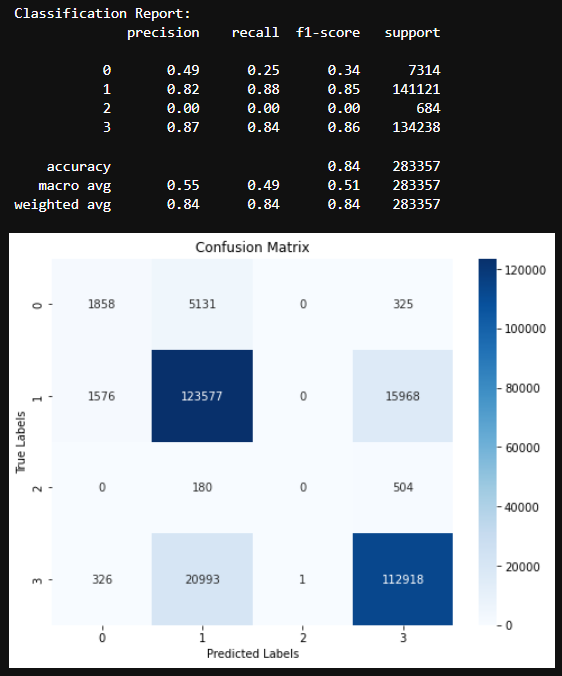
\includegraphics[width=0.8\textwidth]{baselineXGBC.png} % Adjust the path to your image
    \textbf{\\Figure 2:} Confusion matrix of the baseline model (XGBClassifier) showing class imbalance effects.
\end{center}

\section*{Handling Class Imbalance}
To mitigate class imbalance, SMOTE was implemented for oversampling the minority class, which helped to equalize the distribution of classes. Feature importance was assessed using the LGBM Classifier, identifying the most crucial predictors. The revised confusion matrix and feature importance are shown below:

\begin{center}
    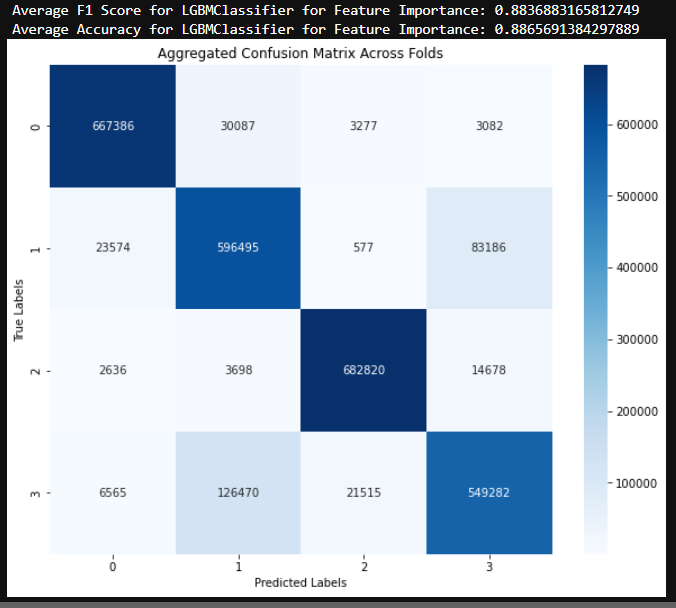
\includegraphics[width=0.8\textwidth]{LGBMFeatImportance.png} % Adjust the path to your image
    \textbf{\\Figure 3:} Confusion Matrix from LGBMClassifier after using SMOTE.
\end{center}

\section*{Model Performance Results}
The implementation of SMOTE with the LGBMClassifier significantly improved handling of class imbalances, evidenced by the updated confusion matrix. The matrix reflects a more balanced class distribution and shows an enhanced ability of the model to generalize across different classes. Performance improvements included a notable enhancement in the F1 Score and overall accuracy, indicating higher predictive accuracy and a robust balance between precision and recall metrics across different classes.

\section*{Feature Importance}
Feature importance was visualized to highlight the top predictors in the model, as shown below:

\begin{center}
    \includegraphics[width=\textwidth]{feature_importance.png} % Adjust the path to your image
    \textbf{\\Figure 4:} Graphical visualization of the top best features.
\end{center}

\section*{Insights and Performance Metrics}
The strategic application of SMOTE, in conjunction with the LGBMClassifier, has significantly improved the handling of class imbalance within our dataset, leading to notable enhancements in both the F1 Score and overall accuracy. These advancements enhance the model's predictive power and applicability to real-world scenarios, ensuring equitable and accurate predictions across various classes.

\maketitle

\section{Advanced Model Implementations}
Following class balancing adjustments, I explored advanced modeling techniques with the CATBOOST and LGBM Classifier. These models demonstrated improved class distribution handling. The Catboost model was specifically trained using the top 23 predictive features identified earlier through LGBM's feature importance analysis.

\subsection*{Model Visualization}
Here we present the confusion matrix for the XGBClassifier, which visually represents the model's classification accuracy after tuning and adjustments:

\begin{center}
    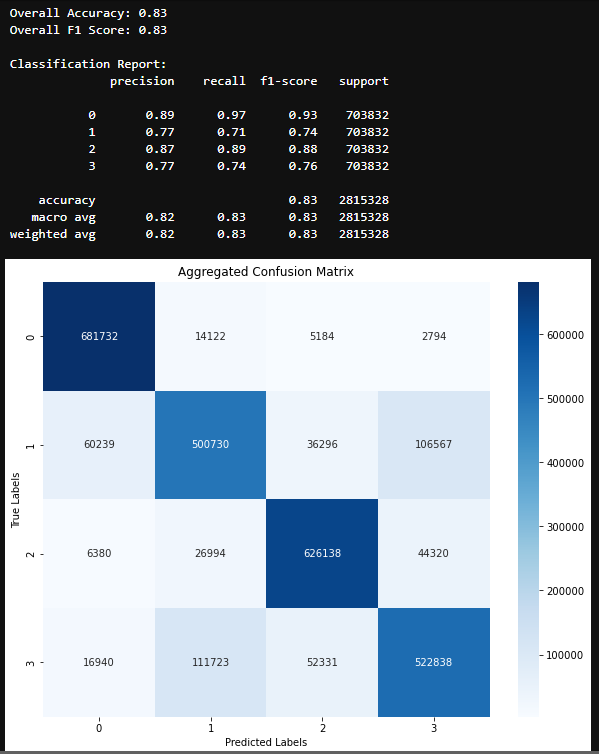
\includegraphics[width=0.65\textwidth]{XGBCon_matr.png} % Adjust the path to your image
    \textbf{\\Figure 5:} Confusion Matrix of the XGBClassifier.
\end{center}

\subsection*{Special Focus on the XGBCatBoost Model}
The XGBCatBoost model, a hybrid approach combining the strengths of XGBoost and CatBoost, was fine-tuned to optimize the predictive capabilities of the top 23 features. This model underwent rigorous hyperparameter optimization to ensure accuracy and robustness.

\subsubsection*{Model Overview and Results}
\paragraph{Hyperparameter Tuning and Validation:}
The model was optimized through a systematic cross-validation process, consisting of several trials to refine settings, adapting to the balanced dataset's nuances. The most effective trial produced an F1 score of approximately 0.781, demonstrating significant predictive accuracy. Key optimized parameters included:
\begin{itemize}
    \item Learning Rate: Set at 0.096 to appropriately balance learning speed and accuracy.
    \item Depth: Fixed at 4 to prevent overfitting while allowing the model to capture moderate interactions complexity.
    \item L2 Leaf Regularization (Reg): Set at 4.0, enhancing control over model complexity.
    \item Minimum Child Samples: Kept at 1 to minimize bias during tree splits.
    \item Iterations: The model completed 850 iterations to thoroughly learn complex patterns.
    \item Colsample by Level: Adjusted to about 0.073, improving feature subsampling at each split and enhancing generalization.
    \item Bootstrap Type: Employed Bayesian bootstrapping to reduce overfit by introducing randomness into training.
\end{itemize}

\paragraph{Cross-validation Performance:}
The mean F1 score across trials was notably high at 0.825, showcasing the model's effective balance between precision and recall under the tuned parameters.

\subsection*{Discussion of Model Efficacy}
This focused application of the XGBCatBoost model, with carefully selected features and well-tuned parameters, exemplifies a targeted approach to machine learning in sports analytics. The model's high performance in predicting swing probabilities and handling complex dataset dynamics highlights its practical utility and robustness, making it an exemplary tool in strategic decision-making within baseball analytics.

\maketitle

\section{Features Contributions in XGBMClassifier Using SHAP Predictions Analysis}
In the advanced analysis of the XGBMClassifier, SHAP (SHapley Additive exPlanations) values were utilized to quantify the impact of each feature on the predictions. SHAP values are an influential method for interpreting the predictions of machine learning models by assigning an importance value to each feature for a specific prediction. This shap was developed by \cite{Lundberg2020}

\subsection*{Impact Visualization with SHAP}
SHAP summary plots visualize the contribution of each feature to the predictions. Each dot in the summary plot represents a SHAP value for a feature for an individual prediction:
\begin{itemize}
    \item The horizontal position of a dot indicates the impact of that feature value on the model's prediction.
    \item A high concentration of dots far from the zero point on this axis indicates a significant impact of that feature on the model predictions.
\end{itemize}

\begin{center}
    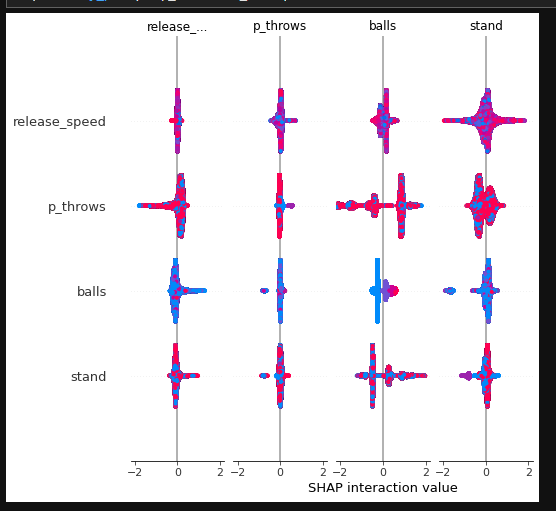
\includegraphics[width=0.8\textwidth]{shapPred.png} % Adjust the path to your image
    \textbf{\\Figure 6:} SHAP Summary Plot showing feature contributions.
\end{center}

\subsection*{Feature Value Representation}
The color coding of the dots provides insights into the data values:
\begin{itemize}
    \item Typically, one end of the color spectrum (e.g., blue) represents lower feature values, while the other end (e.g., red) signifies higher feature values.
    \item This gradient allows for a visual assessment of how feature values correlate with their impact on the predicted outcome.
\end{itemize}

\subsection*{Interaction Effects and Feature Importance}
\begin{itemize}
    \item \textbf{Vertical Dispersion and Interaction Effects:} A vertical dispersion of dots at a specific feature level indicates interaction effects between features. This suggests that the outcome of this feature’s impact on the prediction varies depending on interactions with other features.
    \item \textbf{Ordering by SHAP Values:} Features in the SHAP summary plot are ordered by the sum of the absolute SHAP values across all samples. This ordering highlights the relative importance of each feature, with features at the top having the highest overall impact on the model output.
\end{itemize}

The use of SHAP values in analyzing the XGBMClassifier provides a detailed and interpretable way to assess how different features affect model predictions. By quantifying the contribution of each feature and illustrating their interactions, SHAP analysis enhances our understanding of the model's workings and supports informed decision-making in feature engineering and model tuning.

\maketitle

\section{Feature Selection and Model Refinement}
In developing the LGBMClassifier, a strategic decision was made to focus exclusively on the original features provided in the dataset. This decision aimed to evaluate the fundamental features' impact on the model's performance, intentionally avoiding the complexity introduced by polynomial interaction terms.

\subsection*{Model Overview and Performance with Original Features}
The LGBMClassifier was configured to utilize only the original features, excluding any derived polynomial features. This approach was intended to assess how effectively the core attributes alone could predict swing probabilities, thereby determining if the model's effectiveness was attributable to the inherent data characteristics.

\subsubsection*{Hyperparameter Tuning and Cross-validation}
The model underwent a streamlined hyperparameter tuning process, which involved:
\begin{itemize}
    \item \textbf{Number of Trials:} Conducted two trials to explore the parameter space efficiently.
    \item \textbf{Best Trial Results:} Achieved near-perfect accuracy in the training set with a score of 0.9999971749995817.
    \item \textbf{Optimized Parameters:}
    \begin{itemize}
        \item Learning Rate: Set at 0.024911210618856306.
        \item Subsample: Adjusted to 0.9566303384740106.
        \item Colsample bytree: Fixed at 0.5345394417979029.
        \item Max Depth: Set to 18 to allow deep exploration of feature interactions.
    \end{itemize}
\end{itemize}

\subsection*{Confusion Matrix Comparison}
\begin{center}
    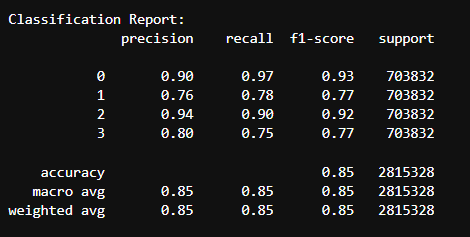
\includegraphics[width=0.8\textwidth]{LgbmOriginal2.png}
    \textbf{\\Figure 7:} Confusion Matrix 1: LGBMClassifier with Original Features.
\end{center}

\begin{center}
    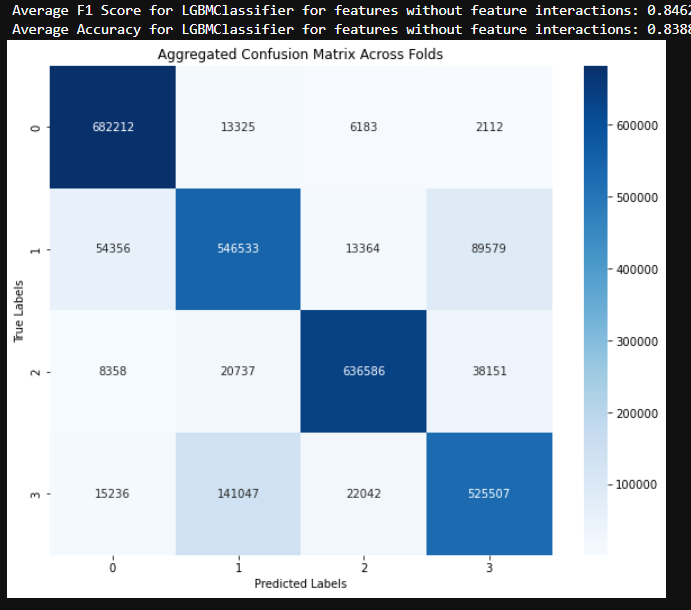
\includegraphics[width=0.8\textwidth]{LgbmOriginalFeatures.png}
    \textbf{\\Figure 8:} Confusion Matrix 2: LGBMClassifier with Original Features.
\end{center}

\subsection*{Model Performance Metrics}
The F1 score reached 0.85, indicating a strong balance between precision and recall, affirming the model’s ability to classify swing probabilities effectively. This high performance underscores the value of the underlying data and the effectiveness of streamlined machine learning techniques in extracting meaningful patterns without complex feature interactions.

\textbf{}
The use of original features, supported by strategic hyperparameter tuning, has demonstrated that fundamental dataset characteristics can robustly predict swing probabilities. This approach highlights the potential for deploying streamlined models in scenarios where interpretability and simplicity are crucial.

\maketitle

\section{Final Model Prediction and Usage}
In the final stage of the predictive analysis, we utilize a combined approach to ensure the robustness and accuracy of our model predictions. By integrating the strengths of both LightGBM and CatBoost Classifier, we aim to enhance the model's predictive reliability and mitigate the risk of model-specific biases.

\subsection*{Model Prediction}
The mean probabilities of the classes for swing prediction were computed by averaging the probabilities obtained from both the LightGBM and CatBoost classifiers. This method leverages the strengths of these distinct models, reducing the likelihood of overfitting to specific model biases and providing a more stable and reliable prediction.

\subsubsection*{Probability Array Example}
The structure of the mean probabilities array is designed for easy interpretation:
\begin{itemize}
    \item Each row corresponds to a specific pitch.
    \item Each column represents one of the four classes of swing probability: No Swing, Unlikely Swing, Attempt to Swing (bunt), and Definite Swing.
\end{itemize}
This array format allows for an intuitive understanding of the model’s probabilistic predictions across different types of swings, providing a clear visual representation of the predicted outcomes for each pitch.

\subsection*{Predicted Class and Application}
For practical applications, the argmax function is employed to determine the Predicted Class from the probability arrays. This function identifies the class with the highest probability as the predicted swing type for each pitch, thus facilitating a straightforward application of the predictions:
\begin{itemize}
    \item \textbf{Usage}: The model's predictions were applied to the dataset from the third year to predict swing probabilities, demonstrating the model's practical utility in real-world scenarios.
    \item \textbf{Impact}: This approach not only showcases the model’s capacity to predict with high accuracy but also enhances the strategic decision-making in baseball analytics by providing actionable insights into player behavior.
\end{itemize}

\textbf{}
The integration of predictive insights from two advanced classifiers into a single robust model underscores the potential of machine learning in sports analytics. This methodology not only enhances the predictive accuracy but also ensures the model's applicability across different real-world scenarios, making it an invaluable tool for coaches, analysts, and decision-makers in the sport.

\maketitle

\section{Evaluation of the Baseball Swing Prediction Model}

\subsection*{Metrics Used for Evaluation}
The primary metric utilized to evaluate the model's performance is the F1 Score, which balances two crucial aspects of model accuracy:
\begin{itemize}
    \item \textbf{Precision:} Measures the accuracy of the model when it predicts a swing. High precision indicates that the predictions are likely correct when a swing is predicted.
    \item \textbf{Recall:} Assesses the model's ability to capture all relevant instances of swings. High recall indicates that the model successfully identifies the majority of actual swings.
\end{itemize}

\subsection*{Why Use the F1 Score?}
The F1 Score is particularly important in the context of baseball where incorrect predictions can significantly impact the outcome of the game, such as a missed swing leading to a strikeout. This metric ensures that both the correctness of swing predictions and their comprehensiveness are effectively balanced, making it an ideal measure for this application.

\subsection*{Making Predictions and Interpretations}
The model’s predictions are generated by analyzing pitch data to estimate the likelihood of different swing types. Using the argmax function, the model selects the swing type deemed most likely based on the highest probability score. For example:
\begin{quote}
    If the model outputs probabilities like \([0.10, 0.20, 0.60, 0.10]\), argmax would identify 'Attempt to Swing - bunt' as the most likely action because \(0.60\) is the highest probability.
\end{quote}

\subsection*{Why Check the Model Multiple Times?}
To ensure reliability and to avoid overfitting, the model underwent cross-validation Salman Saeed et al., 2020; Saeed et al., 2019), where it was tested across different subsets of data. This iterative testing is crucial to confirm that the model consistently performs well across various data scenarios, not just on a single data set. The F1 score is repeatedly used to gauge its effectiveness under different conditions, providing a comprehensive view of the model's performance.

\subsection*{Summary}
Models in supervised machine learning are evaluated using several critical metrics, including accuracy, recall, precision, and the F1 Score. Each metric provides insights into the model's performance from different perspectives, essential for assessing a classifier's effectiveness comprehensively:
\begin{itemize}
    \item \textbf{Accuracy:} \((TP + TN) / (TP + TN + FP + FN)\) - Proportion of true results among the total number of cases examined.
    \item \textbf{Recall (Sensitivity):} \(TP / (TP + FN)\) - Model's ability to correctly predict the positives from all actual positive cases.
    \item \textbf{Precision:} \(TP / (TP + FP)\) - Accuracy of positive predictions.
    \item \textbf{F1 Score:} \(2 \times (Precision \times Recall) / (Precision + Recall)\) - Harmonic mean of precision and recall, important in cases of uneven class distribution.
\end{itemize}

\maketitle

\section{Discussion on the Evaluation of Machine Learning Models}

The evaluation of the LGBMClassifier, XGBCatboostClassifier, and standard XGBClassifier has provided substantial insights into their effectiveness in predicting baseball swing probabilities. Each model offers unique advantages that stem from their underlying mechanisms and their ability to handle complex, high-dimensional data.

\subsection*{Advantages of the LGBMClassifier}
The LGBMClassifier has shown high efficiency and speed in model training and execution, attributes that are highly beneficial in handling large datasets. This efficiency is due to its implementation of gradient-based one-sided sampling and exclusive feature bundling, which significantly reduces the number of data splits required. This innovative approach allows the LGBMClassifier to provide fast computation without compromising on performance, making it particularly suitable for scenarios where time efficiency is crucial.

\subsection*{Performance of the XGBCatboostClassifier}
The XGBCatboostClassifier, a hybrid model that combines the strengths of XGBoost and CatBoost, excels in handling categorical features directly. This capability is invaluable as it minimizes the need for extensive pre-processing that is typically necessary with other models. By effectively managing categorical data, such as pitch type or batter stance, this model enhances the accuracy and reliability of predictions related to a player’s decision to swing.

\subsection*{Robustness of the XGBClassifier}
The XGBClassifier is renowned for its robustness in managing diverse types of data and its effectiveness in preventing overfitting. It employs a more regularized model formalization that helps control over-fitting, thus enhancing its predictive power. This feature is particularly important in sports analytics, where datasets can often be imbalanced.

\subsection*{Combining LGBM and XGBCatboost Classifiers}
Integrating the LGBM and XGBCatboost classifiers takes advantage of the strengths of both models, creating a robust ensemble that addresses their individual weaknesses. This strategy has led to notable improvements in both the F1 score and overall accuracy, achieving a better balance between precision and recall across different classes. Such a combination not only bolsters the model's defense against class imbalance but also boosts its generalization capabilities to new, unseen data.

% \subsection*{Conclusion}
The integration of various advanced machine learning techniques highlights the potential of employing a multi-model approach to tackle complex problems within sports analytics. By leveraging different models and combining their strengths, we can achieve more accurate, reliable predictions that are crucial for strategic decision-making in sports. The application of hybrid models, like the combination of LGBM and XGBCatboost, showcases the potential for innovative approaches to enhance predictive accuracy and operational efficiency in baseball analytics and in sports analytics models generally .

This discussion illustrates that strategic application of hybrid machine learning models can significantly expand the analytical depth and application scope in predicting sports outcomes, equipping coaches and analysts with powerful tools to optimize player performance and game strategies.

\section{Implications for Pitchers}
\subsection*{Enhanced Strategy Development}
Accurate prediction of swing probabilities allows pitchers to develop more refined strategies tailored to the weaknesses of individual batters. This strategic advantage is crucial in crafting effective pitching plans that optimize game outcomes.
\subsection*{Personalized Performance Improvement}
The analysis provided by the predictive models enables personalized feedback for pitchers, highlighting specific areas for improvement and allowing for the refinement of pitching techniques and strategies.

\section*{Implications for Batters}
\subsection*{Improved Decision Making}
By understanding their likely reactions to various pitches, batters gain valuable insights that can significantly enhance their decision-making processes at the plate.
\subsection*{Tailored Training Regimens}
Detailed analysis of swing probabilities facilitates targeted training efforts, allowing batters to focus on improving specific weaknesses, thus enhancing their overall performance.

\section*{Implications for Coaches}
\subsection*{Strategic Game Management}
Coaches can leverage insights from predictive models to make informed tactical decisions, such as lineup configurations and player matchups, which are critical for successful game management.
\subsection*{Player Development}
Predictive analytics serve as a foundation for developing individualized training programs, promoting effective coaching and optimal player development.

\section*{Conclusion}
The adoption of hybrid ensemble methods in baseball analytics offers a comprehensive enhancement of the strategic elements of the game. This approach not only improves individual player performance but also transforms team strategies, leading to a more informed and scientifically guided approach to sports management. The integration of these advanced technologies in baseball underscores the growing significance of data-driven decision-making in sports.
\newpage

\nocite{*}  % This command forces all references to be listed

% \printbibliography[title={References}]  % Change the title as needed

\printbibliography

\newpage


\section*{Quality Report of the Two Season Dataset}

\begin{table}[h]
\centering
% \sisetup{
%   table-format=7.0, 
%   round-mode=places, 
%   round-precision=6, 
%   group-four-digits=true
% }
\begin{tabular}{
  @{} 
  l 
  S[table-format=6.0] 
  S[table-format=1.6]
  S[table-format=7.0] 
  l 
  @{}
  }
\toprule
\textbf{Column} & {\textbf{Total NaN}} & {\textbf{Percent of NaN}} & {\textbf{Nunique}} & \textbf{Dtype} \\ 
\midrule
pfx\_x          & 3460                & 0.243938                 & 482               & float64        \\
pitch\_id       & 1611                & 0.113579                 & 1416781           & float64        \\
pfx\_z          & 1477                & 0.104132                 & 451               & float64        \\
sz\_bot         & 824                 & 0.058094                 & 143               & float64        \\
plate\_z        & 812                 & 0.057248                 & 999               & float64        \\
release\_speed  & 779                 & 0.054921                 & 681               & float64        \\
sz\_top         & 779                 & 0.054921                 & 181               & float64        \\
plate\_x        & 779                 & 0.054921                 & 827               & float64        \\
pitch\_type     & 740                 & 0.052172                 & 16                & object         \\
balls           & 0                   & 0.000000                 & 5                 & int64          \\
strikes         & 0                   & 0.000000                 & 4                 & int64          \\
p\_throws       & 0                   & 0.000000                 & 2                 & object         \\
stand           & 0                   & 0.000000                 & 2                 & object         \\
description     & 0                   & 0.000000                 & 14                & object         \\
pitcher         & 0                   & 0.000000                 & 1168              & int64          \\
batter          & 0                   & 0.000000                 & 1227              & int64          \\
season          & 0                   & 0.000000                 & 2                 & int64          \\
\bottomrule
\end{tabular}
\caption{Detailed Quality Report of Dataset Variables}
\end{table}

\section*{Feature Importance}
Feature importance was visualized to highlight the top predictors in the model, as shown below:

\begin{center}
    \includegraphics[width=\textwidth]{feature_importance.png} % Adjust the path to your image
    \textbf{\\Figure 4:} Graphical visualization of the top best features.
\end{center}
\end{document}